\documentclass[tikz,border=10pt]{standalone}
\usetikzlibrary{arrows.meta, decorations.pathreplacing}

\tikzset{
    axis/.style={->,thick},
    grid/.style={thin,dotted},
    function/.style={blue,solid},
    function-dashed/.style={red,dashed}
}

\begin{document}
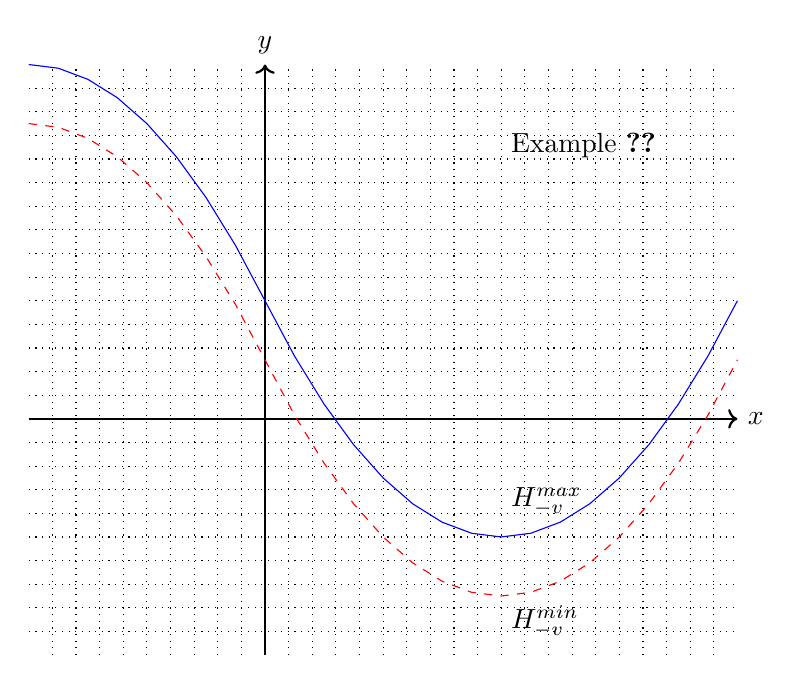
\begin{tikzpicture}[scale=1.5]

% Draw axes
\draw[axis] (-2,0) -- (4,0) node[right] {$x$};
\draw[axis] (0,-2) -- (0,3) node[above] {$y$};

% Draw grid
\foreach \x in {-1.8,-1.6,...,3.8}{\draw[grid] (\x,-2) -- (\x,3);}
\foreach \y in {-1.8,-1.6,...,2.8}{\draw[grid] (-2,\y) -- (4,\y);}

% Draw functions
\draw[function] plot[domain=-2:4] ({\x},{0.5*\x^2 - 2*\x + 1});
\draw[function-dashed] plot[domain=-2:4] ({\x},{0.5*\x^2 - 2*\x + 0.5});

% Add labels
\node at (2,2.5) [below right] {Example~\ref{ex:facefan2}};
\node at (2,-0.5) [below right] {$H_{-v}^{max}$};
\node at (2,-1.5) [below right] {$H_{-v}^{min}$};

\end{tikzpicture}
\end{document}